\section{Introdução}
O termo \textbf{sistema legado} descreve um sistema antigo que permanece em operação em uma organização onde geralmente utilizam bancos de dados obsoletos.

Normalmente são aplicações complexas, de difícil manutenção e, pelo grau de criticidade e custo para modernização, continuam ativas. Por falta de documentação e com a saída do pessoal técnico que participou originalmente no seu desenvolvimento, os sistemas legados podem apresentar problemas como:\footnote{https://pt.wikipedia.org/wiki/Sistema\_legado}:
\begin{itemize}
    \item Dificuldade de compreensão das regras de negócio neles implementadas;
    \item Desconhecimento das razões que levaram a determinadas decisões;
    \item Problemas na estruturação dos módulos de código;
    \item Miscelânea de estilos de programação;
    \item Obsolescência das ferramentas de desenvolvimento;
    \item Impossibilidade de reaproveitamento dos equipamentos nos quais são executados para execução de softwares mais atuais;
\end{itemize}
Ian Warren elenca as seguintes características de sistemas legados:
\begin{itemize}
    \item Altos custos de manutenção;
    \item Software complexo;
    \item Software de suporte obsoleto;
    \item Hardware obsoleto;
    \item Sem conhecimento técnico;
    \item Negócio crítico;
    \item Backlog de solicitações de mudança;
    \item Documentação deficiente;
    \item Conhecimento empresarial incorporado;
    \item Mal compreendido pelos mantenedores;
\end{itemize}

Os sistemas legados existem pois faziam sentido na época em que foram concebidos, mas com novos paradigmas, o conceito de maturidade mudou e estes mesmos sistemas necessitam de ajustes.

\begin{figure}[H]
    \centering
    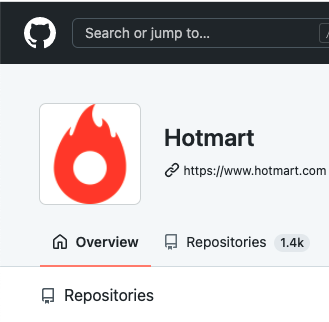
\includegraphics[scale=0.60,keepaspectratio=true]{images/01.png}
    \caption{Processo de maturidade}
    \label{mature_process}
\end{figure}

Na Figura \ref{mature_process}, podemos perceber como a oscilação das escolhas eram muito maiores antes de atingir o ponto de maturidade do que são a partir do momento em que já sabem qual caminho deseja trilhar.

Se fosse possível escolher as melhores partes das escolhas que nos tiraram do ponto de origem e nos levaram ao ponto de maturidade? Este seria um processo chamado de consolidação do conhecimento. Veja na Figura \ref{knwledge_consolidation}.

\begin{figure}[H]
    \centering
    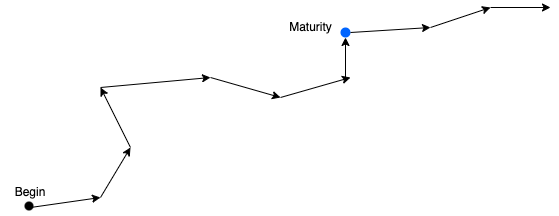
\includegraphics[scale=0.60,keepaspectratio=true]{images/02.png}
    \caption{Processo de consolidação do conhecimento}
    \label{knwledge_consolidation}
\end{figure}

Agora, mesmo que soubéssemos as melhores escolhas, de nada adiantaria chegar até aqui sem a correta manutenção de cada delas, ou seja, sendo cada nova decisão deve-se levar em conta todas as demais.

\begin{figure}[H]
    \centering
    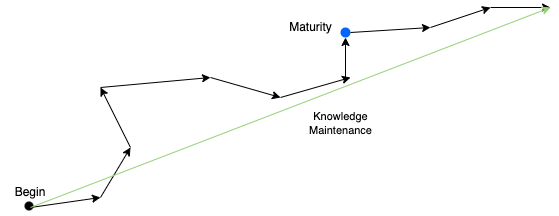
\includegraphics[scale=0.60,keepaspectratio=true]{images/03.png}
    \caption{Processo de manutenção do conhecimento}
    \label{knowledge_maintenance}
\end{figure}

A cada passo de reconstrução, é muito importante documentar todas as etapas como por exemplo, regras de negócio, parâmetros e configurações e até mesmo um livro de receitas\footnote{playbook} que contem fragmentos de códigos que servem como referência futura. Quando temos uma referência em uma linha de produção, fica muito mais fácil garantir a qualidade de um produto.

Neste momento, estaríamos no que chamamos de \textbf{``Estado da Arte''} onde diversos setores da empresa poderiam trabalhar munidos de seus livros de receitas para execução de suas tarefas, entregando um trabalho de qualidade e deixando criatividade para ser utilizada no momento da criação de novos projetos ou seus incrementos.